\section{Decision Trees [20 pts]}
\begin{enumerate}


\item Consider the dataset in Table \ref{dec_tab} for this problem. Given the four attributes on the left, we want to predict if the student got an A in the course. The following questions involve some computation, so you may want to solve them programmatically. You can find this dataset in \textit{data.txt}

\begin{table}[ht]
\begin{center}
\begin{tabular}{| c | c | c | c || c |} 
\hline
\vtop{\hbox{\strut \textbf{Wakes Up}}\hbox{\strut \textbf{Early}}} & \vtop{\hbox{\strut \textbf{Finished All}}\hbox{\strut \textbf{Homework}}} & \vtop{\hbox{\strut \textbf{Completed}}\hbox{\strut \textbf{Pre-requisites}}} & \textbf{Likes Coffee} & \textbf{A} \\ 
\hline
1 & 1 & 0 & 0 & 0\\ 
\hline
1 & 1 & 1 & 0 & 1\\ 
\hline
0 & 0 & 1 & 0 & 0\\ 
\hline
0 & 1 & 1 & 0 & 1\\ 
\hline
0 & 1 & 1 & 0 & 1\\ 
\hline
0 & 0 & 1 & 1 & 0\\ 
\hline
1 & 0 & 0 & 0 & 0\\ 
\hline
0 & 1 & 0 & 1 & 1\\ 
\hline
0 & 0 & 1 & 0 & 1\\ 
\hline
1 & 0 & 0 & 0 & 0\\ 
\hline
1 & 1 & 1 & 0 & 1\\ 
\hline
0 & 1 & 1 & 1 & 0\\ 
\hline
0 & 0 & 0 & 0 & 0\\ 
\hline
1 & 0 & 0 & 1 & 0\\ 
\hline
\end{tabular}
\end{center}
\caption{decision tree features and labels}
\label{dec_tab}
\end{table}

Create a decision tree of depth 2 using the ID3 algorithm from class. The tree should have the same structure as the diagram in Figure~\ref{fig:tree}. Note that 0 leads to the left branch and 1 leads to the right branch. 
\begin{figure}[ht]
\begin{center}
  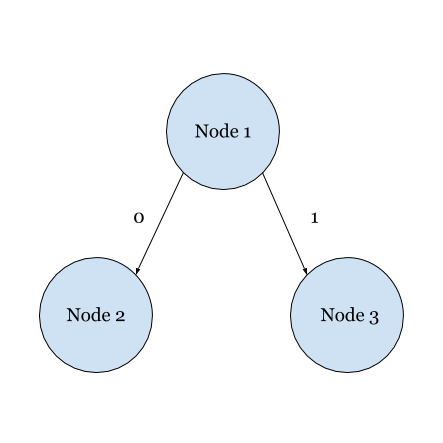
\includegraphics[width=5cm]{images/decisiontree.png}
\end{center}
  \caption{Decision tree structure for question 1}
\label{fig:tree}
\end{figure}
\begin{enumerate}[label=(\roman*)]

\newpage

\item \textbf{[4 pts]} What is the attribute at Node 1? What is the information gain of this attribute? Please round your answer to 4 decimal places.

Attribute to split on: \begin{tcolorbox}[fit,height=1.2cm, width=3.5cm, blank, borderline={1pt}{-2pt}, nobeforeafter, box align = center] \end{tcolorbox}
\hspace{0.5cm} Mutual information: \begin{tcolorbox}[fit,height=1.2cm, width=3.5cm, blank, borderline={1pt}{-2pt}, nobeforeafter, box align = center] \end{tcolorbox} 
 
    
\item \textbf{[4 pts]} What is the attribute at Node 2? What is the information gain of this attribute? Please round your answer to 4 decimal places.

Attribute to split on: \begin{tcolorbox}[fit,height=1.2cm, width=3.5cm, blank, borderline={1pt}{-2pt}, nobeforeafter, box align = center] \end{tcolorbox}
\hspace{0.5cm} Mutual information: \begin{tcolorbox}[fit,height=1.2cm, width=3.5cm, blank, borderline={1pt}{-2pt}, nobeforeafter, box align = center] \end{tcolorbox} 


\item \textbf{[4 pts]} What is the attribute at Node 3? What is the information gain of this attribute? Please round your answer to 4 decimal places. \\
\\
Note: If there is a tie on the attribute with the highest information gain, write any of the attribute that has the highest information gain.

Attribute to split on: \begin{tcolorbox}[fit,height=1.2cm, width=3.5cm, blank, borderline={1pt}{-2pt}, nobeforeafter, box align = center] \end{tcolorbox}
\hspace{0.5cm} Mutual information: \begin{tcolorbox}[fit,height=1.2cm, width=3.5cm, blank, borderline={1pt}{-2pt}, nobeforeafter, box align = center] \end{tcolorbox} 

    
\end{enumerate}

\item \textbf{[4 pts]} Consider learning a decision tree for some binary classification task. Assume that we do not restrict the size of the tree and that the tree can branch multiple times on the same attribute. Under what condition(s) would we be unable to construct a tree that perfectly classifies the dataset?  
\begin{tcolorbox}[fit,height=5cm, width=15cm, blank, borderline={1pt}{-2pt}]

\end{tcolorbox}


\item \textbf{[4 pts]} Given enough time, is the ID3 algorithm guaranteed to output the smallest decision tree that is \emph{consistent} with the training dataset i.e., achieves zero training error rate? Briefly explain why or why not. 
\begin{tcolorbox}[fit,height=5cm, width=15cm, blank, borderline={1pt}{-2pt}]
%solution
\end{tcolorbox}


\end{enumerate}
\newpage

\section{Nearest Neighbors and Decision Trees [6 Points]}

Consider a multiclass classification problem with 2 real-valued features. Suppose you are given $n$ data points $P_1, P_2, \ldots, P_n$ and the corresponding label for each data point $C_1, C_2, \ldots, C_n$ (where $C_1, C_2, \ldots, C_n$ take values from the set of all possible class labels). Under the $k$ nearest neighbors classification scheme, each new element $Q$ is simply categorized by a majority vote among its $k$ nearest neighbors. The 1-NN is a simple variant of this which divides up the input space for classification purposes into convex regions (see Figure \ref{fig:KNN_and_DT}), each corresponding to a point in the dataset.

\begin{figure}[H]
    \centering
    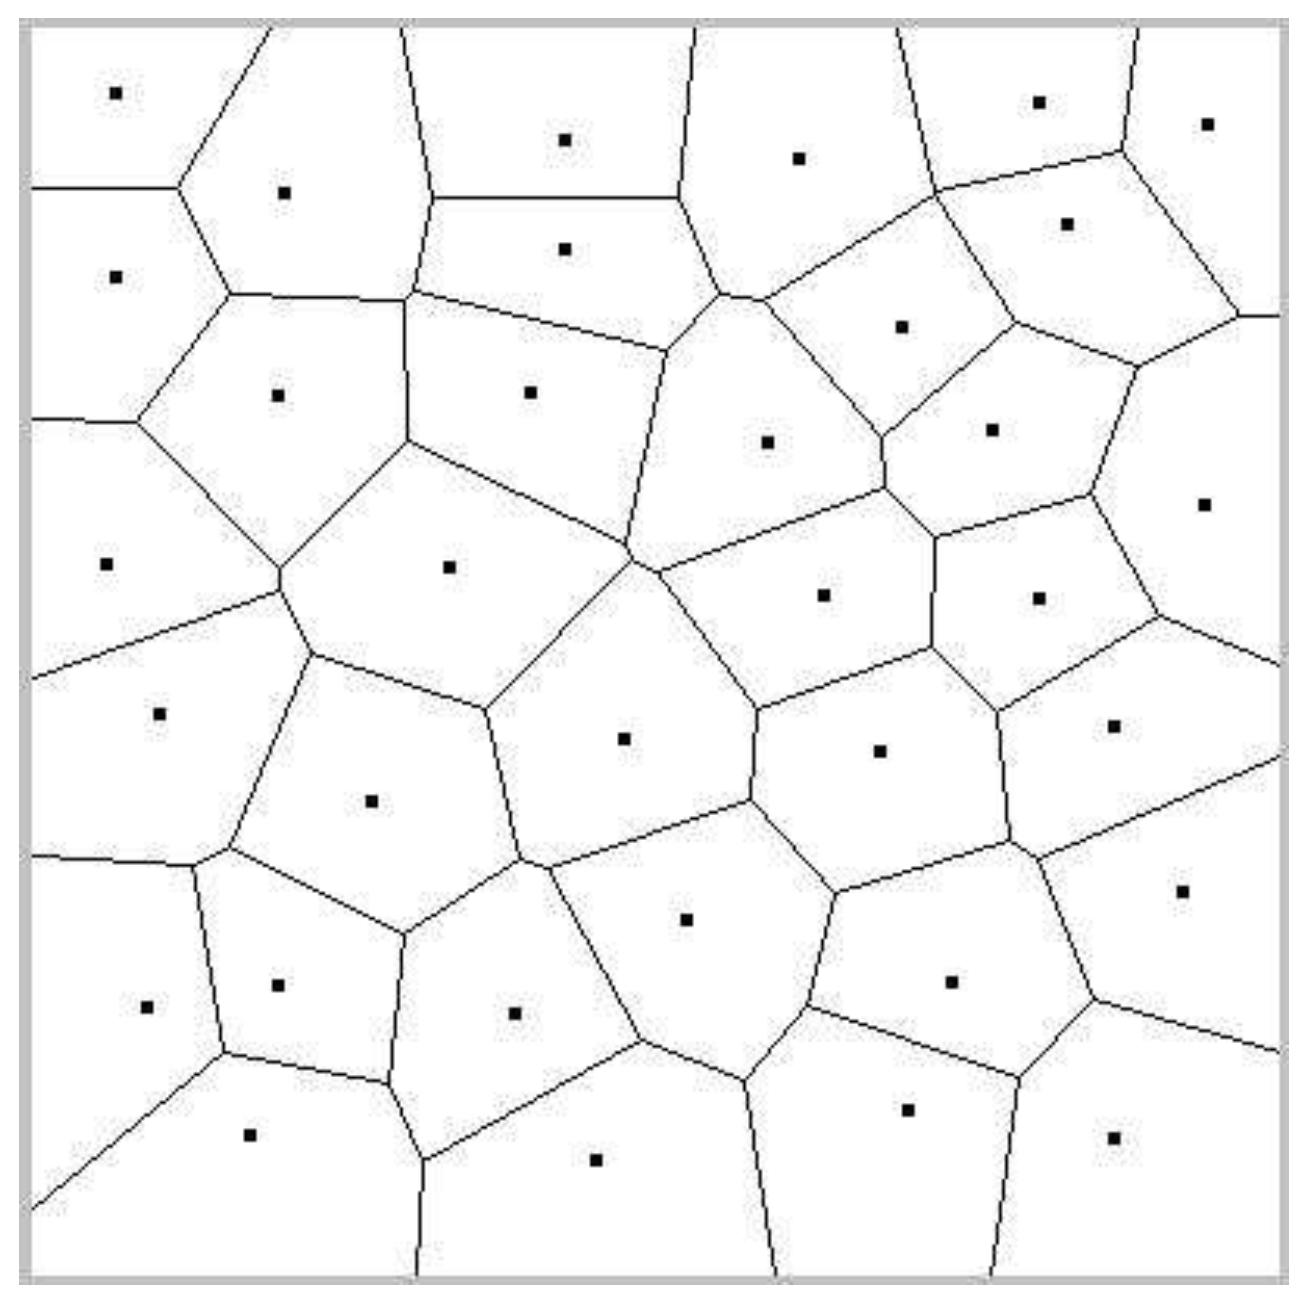
\includegraphics[width=0.5\textwidth]{images/1_KNN_and_DT.png}
    \caption{1-NN decision boundaries using the Euclidean distance metric.}
    \label{fig:KNN_and_DT}
\end{figure}
\begin{enumerate}

\item {\bf [6 Points]} Is it possible to build a decision tree (with decisions at each node of the form ``is $x_1 > a$'', ``is $x_1 < b$'', ``is $x_2 > c$'', or ``is $x_2 < d$'' for any real constants $a,b,c,d$) which behaves identically to a 1-NN classifier using the Euclidean distance metric? If so, how and if not, why not.

\begin{tcolorbox}[fit,height=7cm, width=15cm, blank, borderline={1pt}{-2pt}]

\end{tcolorbox}

\end{enumerate}
\newpage